\documentclass[10pt]{article}
\usepackage{fullpage}
\usepackage{amsmath}
\usepackage[amsthm, thmmarks]{ntheorem}
\usepackage{amssymb}
\usepackage{graphicx}
\usepackage{enumerate}
\usepackage{verse}
\usepackage{tikz}
\usepackage{verbatim}
\usepackage{hyperref}
\usepackage{algpseudocode}
\usepackage{algorithm}

\newtheorem{lemma}{Lemma}
\newtheorem{theorem}[lemma]{Theorem}
\newtheorem{definition}[lemma]{Definition}
\newtheorem{proposition}[lemma]{Proposition}
\newtheorem{corollary}[lemma]{Corollary}
\newtheorem{claim}[lemma]{Claim}
\newtheorem{example}[lemma]{Example}

\newcommand{\dee}{\mathrm{d}}
\newcommand{\Dee}{\mathrm{D}}
\newcommand{\In}{\mathrm{in}}
\newcommand{\Out}{\mathrm{out}}
\newcommand{\pdf}{\mathrm{pdf}}
\newcommand{\Cov}{\mathrm{Cov}}
\newcommand{\Var}{\mathrm{Var}}

\newcommand{\ve}[1]{\mathbf{#1}}
\newcommand{\mrm}[1]{\mathrm{#1}}
\newcommand{\etal}{{et~al.}}
\newcommand{\sphere}{\mathbb{S}^2}
\newcommand{\modeint}{\mathcal{M}}
\newcommand{\azimint}{\mathcal{N}}
\newcommand{\ra}{\rightarrow}
\newcommand{\mcal}[1]{\mathcal{#1}}
\newcommand{\X}{\mathcal{X}}
\newcommand{\Y}{\mathcal{Y}}
\newcommand{\Z}{\mathcal{Z}}
\newcommand{\x}{\mathbf{x}}
\newcommand{\y}{\mathbf{y}}
\newcommand{\z}{\mathbf{z}}
\newcommand{\tr}{\mathrm{tr}}
\newcommand{\sgn}{\mathrm{sgn}}
\newcommand{\diag}{\mathrm{diag}}
\newcommand{\Real}{\mathbb{R}}
\newcommand{\sseq}{\subseteq}
\newcommand{\ov}[1]{\overline{#1}}
\newcommand{\data}{\mathrm{data}}

\DeclareMathOperator*{\argmax}{arg\,max}
\DeclareMathOperator*{\argmin}{arg\,min}


\title{Algorithms for Non-Linear Least Squares}
\author{Pramook Khungurn}

\begin{document}
\maketitle

This note is written as I study algorithms for the non-linear least squares problem, which will culminate in the Levenberg--Marquardt algorithm. Source materials I use for this note includes Madsen \etal~\cite{Madsen:2004}, Henri~\cite{Henri:2024}, Ranganathan~\cite{Ranganathan:2004}, and Norcedal and Wright~\cite{Norcedal:2006}

\section{Notations}

\begin{itemize}
    \item Scalars are denoted by regular (i.e., non-bold, non-italic) small latters: $a$, $b$, $c$, $x$, $y$, and $z$.
    \item We denote vectors with bold, small letters: $\ve{a}$, $\ve{b}$ $\ve{c}$, $\ve{x}$, $\ve{y}$, and $\ve{z}$.
    \item Vector components are denoted with regular, small letters with a subscript. For example, $$\ve{x} = (x_1, x_2, \dots, x_n).$$
    \item Matrices, on the other hand, are denoted by regular, capital letters: $A$, $B$, and $C$.
    \item Scalar functions use the same type face as scalars, and vector functions use the same type face as vectors.
    \item Component functions of vector functions are denoted in the same was a vector components. That is, if $f: \Real^n \ra \Real^m$, then
    \begin{align*}
        \ve{f}(\ve{x}) = \begin{bmatrix} f_1(\ve{x}) \\ f_2(\ve{x}) \\ \vdots \\ f_m(\ve{x}) \end{bmatrix}.
    \end{align*}
    \item For derivatives, we use the notations I developed in a previous note \cite{Khungurn:2022}.
\end{itemize}

\section{Preliminary}

\begin{itemize}
    \item We are interested in solving the {\bf non-linear least squares} problem. That is, we are given a non-linear vector function $\ve{f}: \Real^n \ra \Real^m$, and we want to find $\ve{x}^*$ such that $\| \ve{f}(\ve{x}^*) \|^2$ is minimized. In other words, we want to compute
    \begin{align*}
        \ve{x}^* = \argmin_{\ve{x}} \| \ve{f}(\ve{x}) \|^2.
    \end{align*}

    \item Of course, non-linear least square is a special case of the general {\bf function minimization} problem. Here, we are given a {\bf loss function}, aka an {\bf objective function}, $\mcal{L}: \Real^n \ra \Real$. We want to find
    \begin{align*}
        \ve{x}^* = \argmin_{\ve{x}} \mcal{L}(\ve{x}).
    \end{align*}

    \item Obviously, for the non-linear least square problem, we have that $\mcal{L}(\ve{x}) = \| \ve{f}(\ve{x}) \|^2$.
    
    \item Finding $\argmin_{\ve{x}} \mcal{L}(\ve{x})$ (i.e., the {\bf global minimizer}) is very hard in general, especially with non-linear $\ve{f}$. So, we settle to find a local minimizer instead.
    
    \begin{definition}
        A point $\ve{x} \in \Real^n$ is said to be a {\bf local minimizer} of $\mcal{L}: \Real^n \ra \Real$ if there exists $\delta > 0$ such that $\mcal{L}(\ve{x}') \leq \mcal{L}(\ve{x})$ for all $\| \ve{x} - \ve{x}' \| < \delta$. In other words, there exists a neighborhood of $\ve{x}$ such that $\mcal{L}(\ve{x})$ is minimal.
    \end{definition}

    \item We shall assume that $\mcal{L}$ is differentiable to arbitrary order. As a result, we have that
    \begin{align*}
        \mcal{L}(\ve{x} + \ve{h}) = \mcal{L}(\ve{x}) + \nabla\mcal{L}(\ve{x}) \ve{h} + \frac{1}{2} \ve{h}^T H_{\mcal{L}}(\ve{x}) \ve{h} + O(\| \ve{h} \|^3)
    \end{align*}
    where $H_{\mcal{L}}(\ve{x})$ denotes the Hessian matrix of $\mcal{L}$:
    \begin{align*}
        H_{\mcal{L}}(\ve{x}) = \begin{bmatrix}
            \nabla_{1,1} \mcal{L}(\ve{x}) & \nabla_{1,2} \mcal{L}(\ve{x}) & \cdots & \nabla_{1,n} \mcal{L}(\ve{x}) \\
            \nabla_{2,1} \mcal{L}(\ve{x}) & \nabla_{2,2} \mcal{L}(\ve{x}) & \cdots & \nabla_{2,n} \mcal{L}(\ve{x}) \\
            \vdots & \vdots & \ddots & \vdots \\
            \nabla_{n,1} \mcal{L}(\ve{x}) & \nabla_{n,2} \mcal{L}(\ve{x}) & \cdots & \nabla_{n,n} \mcal{L}(\ve{x})           
        \end{bmatrix}
        = \nabla((\nabla \mcal{L}(\ve{x}))^T).
    \end{align*}

    \item \begin{definition}
        A point $\ve{x} \in \Real^n$ is said to be a {\bf stationary point} of $\mcal{L}: \Real^n \ra \Real$ if $\nabla{L}(\ve{x}) = \ve{0}^T$.
    \end{definition}

    \item \begin{theorem}
        A local minimizer of $\mcal{L}$ is a stationary point.
    \end{theorem}
    In other words, being a staionary point is a necessary condition for being a local minimizer. It is not a sufficient condition because a stationary point can be a \emph{local maximizer} or a \emph{saddle point}      

    \item The sufficient condition for a local minimizer is given below.
    \begin{theorem}
        If $\ve{x}$ is a stationary point of $\mcal{L}$, and $H_{\mcal{L}}(\ve{x})$ is positive definite, then $\ve{x}$ is a local minimizer.
    \end{theorem}
\end{itemize}

\section{Descent Methods}

\begin{itemize}
    \item In this section, we present methods for the general function minimzation problem. We will deal with methods specific to non-linear least squares in the sections after this one.
    
    \item The methods in this section are iterative.
    \begin{itemize}
        \item Start with a starting point $\ve{x}^{(0)}$.
        \item We produce a series of points $\ve{x}^{(1)}$, $\ve{x}^{(2)}$, $\dotsc$.
    \end{itemize}
    Then, we pray that the series of points would converge to a local minimizer $\ve{x}^*$.

    \item Let $\ve{e}^{(k)} = \ve{x}^{(k)} - \ve{x}^*.$ The optimization process converges if $\lim_{k \ra \infty} \| \ve{e}^{(k)}\| = 0$.
    
    \item We are interested in quantifying how the optimization process converges. The speed at which it converges can be measured by how much $\| \ve{e}^{(k+1)} \|$ becomes smaller than $\| \ve{e}^{(k)} \|$. There are multiple types of convergence
    \begin{itemize}
        \item {\bf Linear convergence} is when $\| \ve{e}^{(k+1)}\| \leq a\| \ve{e}^{(k)} \|$ for some $0 < a < 1$ for all $k$ large enough.
        \item {\bf Quadratic convergence} is when $\| \ve{e}^{(k+1)}\| = O(\| \ve{e}^{(k)} \|^2)$ for all $k$ large enough that $\| \ve{e}^{(k)} \|$ is small.
        \item {\bf Superlinear convergence} is when $\| \ve{e}^{(k+1)}\| / \| \ve{e}^{(k)}\| \ra 0$ as $k \ra \infty$.
    \end{itemize}

    \item Most methods try to ensure the \emph{descending condition}
    \begin{align*}
        \mcal{L}(\ve{x}^{(k+1)}) < \mcal{L}(\ve{x}^{(k)})
    \end{align*}
    for all $k \geq 0$. This prevents convergence to a local maximizer. However, we might still end up at a saddle point, but it is quite unlikely because a saddle point has directions that would increase the loss function's value. A {\bf descent method} is one that tries to maintain the descending condition.

    \item All methods in this note is a descent method with a particular structure. In each iteration of such a method, we do the following.
    \begin{itemize}
        \item Find a direction $\ve{h}$ along which to move $\ve{x}^{(k)}$. (Here, $k$ is the index of the iteration.)
        \item Find the step length to move $\ve{x}^{(k)}$.
    \end{itemize}
    
    \item The outline of the descent method is given in Algorithm~\ref{algo:descent-method}.
    
    \begin{algorithm}[t]
    \begin{algorithmic}
        \State $k \gets 0$
        \State $found \gets \mathbf{false}$
        \State $\ve{x} \gets \ve{x}^{(0)}$
        \While {$(\mathbf{not}\ found)$ {\bf and} $(k < k_{\max})$}
            \State $\ve{h} \gets \Call{Find-Direction}{\ve{x}}$
            \If {(no such $\ve{h}$ exists)}
                \State $found \gets \mathbf{true}$
            \Else
                \State $\alpha \gets \Call{Compute-Step-Length}{\ve{x}, \ve{h}}$
                \State $\ve{x} \gets \ve{x} + \alpha\ve{h}$
                \State $k \gets k+1$
            \EndIf
        \EndWhile
    \end{algorithmic}
    \caption{Descent method}
    \label{algo:descent-method}
    \end{algorithm}

    \item Consider how the value of $\mcal{L}$ changes after the update.
    \begin{align*}
        \mcal{L}(\ve{x} + \alpha \ve{h}) 
        &= \mcal{L}(\ve{x}) + \alpha \nabla \mcal{L}(\ve{x}) \ve{h} + O(\alpha^2) 
        \approx \mcal{L}(\ve{x}) + \alpha \nabla \mcal{L}(\ve{x}) \ve{h}
    \end{align*}
    when $\alpha$ is small enough. 
    
    \item \begin{definition}
        A direction $\ve{h}$ is a {\bf descent direction} if $\nabla \mcal{L}(\ve{x}) \ve{h} < 0$.
    \end{definition}

    \item If we are at $\ve{x}$ where there exists no descent direction, it must be that $\nabla \mcal{L}(\ve{x}) = \ve{0}$, so $\ve{x}$ is a stationary point.
    
    \item If there is a descent direction, we then have to find the step length $\alpha$ such that $\mcal{L}(\ve{x} + \alpha \ve{h}) < \mcal{L}(\ve{x}).$ 
\end{itemize}

\subsection{Gradient Descent}

\begin{itemize}
    \item One of the most popular descent method is {\bf gradient descent}. It choose $\ve{h} = -(\nabla \mcal{L}(\ve{x}))^T$  and $\alpha$ to be a fixed small constant.
    
    \item The choice of the descent direction is the best choice locally at $\ve{x}^{(k)}$.
    
    \item However, the convergence of gradient descent is linear and often very slow.
    
    \item Nevertheless, it offers good performance when $\ve{x}$ is far away the converged solution $\ve{x}^*$. So, it is often used as the initial phase of the iterative optimization process.
\end{itemize}

\subsection{Newton's Method}

\begin{itemize}
    \item If $\ve{x}^*$ is a stationary point then, $\nabla \mcal{L}(\ve{x}^*) = \ve{0}$.
    
    \item We also have that
    \begin{align*}
        \nabla \mcal{L}(\ve{x} + \ve{h})^T
        &= \nabla \mcal{L}(\ve{x})^T + \nabla(\nabla \mcal{L}(\ve{x})^T) \ve{h} + O(\| \ve{h} \|^2) \\
        &= \nabla \mcal{L}(\ve{x})^T + H_{\mcal{L}}(\ve{x}) \ve{h} + O(\| \ve{h} \|^2) \\
        &\approx \nabla \mcal{L}(\ve{x})^T + H_{\mcal{L}}(\ve{x}) \ve{h}
    \end{align*}
    when $\| \ve{h} \|$ is small enough.

    \item Assuming that we can get to the stationary point in one step, it must be the case that $\nabla \mcal{L}(\ve{x} + \ve{h})^T = \ve{0}$. So,
    \begin{align*}
        \ve{0} &\approx \nabla \mcal{L}(\ve{x})^T + H_{\mcal{L}}(\ve{x}) \ve{h}.
    \end{align*}
    We go one step further and assume that the above inequality is an equality.
    \begin{align*}
        \ve{0} &= \nabla\mcal{L}(\ve{x})^T + H_{\mcal{L}}(\ve{x}) \ve{h}.
    \end{align*}
    This gives
    \begin{align*}
        \ve{h} = - (H_{\mcal{L}}(\ve{x}))^{-1} \nabla\mcal{L}(\ve{x})^T.
    \end{align*}

    \item {\bf Newton's method} chooses $\ve{h} = - (H_{\mcal{L}}(\ve{x}))^{-1} \nabla\mcal{L}(\ve{x})^T$ and $\alpha = 1$.
    
    \item If $H_{\mcal{L}}(\ve{x})$ is positive definite, we have that
    \begin{align*}
        0 < \ve{h}^T H_{\mcal{L}}(\ve{x}) \ve{h}.
    \end{align*}
    Because of our choice of $\ve{h}$, we have that $H_{\mcal{L}}(\ve{x}) \ve{h} = -\mcal{L}(\ve{x})^T$. As a result,
    \begin{align*}
        0 &< - \ve{h}^T \mcal{L}(\ve{x})^T \\
        \mcal{L}(\ve{x})^T \ve{h} &< 0.
    \end{align*}
    As a result, $\ve{h}$ is a descent direction if $H_{\mcal{L}}(\ve{x})$ is positive definite.

    \item Newton's method is good at a late stage of the optimization process. That is, whne $\ve{x}$ is close to $\ve{x}^*$. If $\ve{x}^*$ is a local minimizer, then $H_{\mcal{L}}(\ve{x}^*)$ is positive definite. As a result, there is a neighborhood around $\ve{x}^*$ such that, if $\ve{x}$ is in that neighborhood, then $H_{\mcal{L}}(\ve{x})$ is also positive definite. As a result, we have that $\ve{h}$ is a descent direction. Moreover, the convergence in this neighborhood is quadratic.
    
    \item On the other hand, if the $H_{\mcal{L}}(\ve{x}^*)$ is negative definite, then $\ve{h}$ will be an \emph{ascent} direction, and the algorithm would converge to a local maximizer at a qudratic rate as well. To prevent this, we should always ensure that each update results in a decrease of the loss function.
    
    \item We can build a hybrid method between gradient descent and Newton's method with the following simple rule. If $H_{\mcal{L}}(\ve{x})$ is positive definite, then we use Newton's method for the current optimization step. Otherwise, we use gradient descent. The pseudocode is given in Algorithm~\ref{algo:hybrid-newton-gradient-descent}.
    
    \begin{algorithm}[t]
    \begin{algorithmic}
        \If {$H_{\mcal{L}}(\ve{x})$ is postiive definite}
            \State $\ve{h} \gets - (H_{\mcal{L}}(\ve{x}))^{-1} \nabla\mcal{L}(\ve{x})^T$
            \State $\alpha \gets 1$
        \Else
        \State $\ve{h} \gets - \nabla\mcal{L}(\ve{x})^T$
        \State $\alpha \gets $ small positive constant
        \EndIf
    \end{algorithmic}
    \caption{A hybrid method between Netwon's and gradient descent}
    \label{algo:hybrid-newton-gradient-descent}
    \end{algorithm}

    \item We can check whether a matrix is positive definite by performing the Cholesky factorization, which, if successful, would imply that the matrix is positive definite and also give us a factorization to compute $- (H_{\mcal{L}}(\ve{x}))^{-1} \nabla\mcal{L}(\ve{x})^T$. Factorization takes $O(n^3)$ where $n$ is the number dimension of $\ve{x}$.
\end{itemize}

\subsection{Line Search}

\begin{itemize}
    \item We see that, in the last two sections, the choice of the step length $\alpha$ does not always work.
    \begin{itemize}
        \item For gradient descent, a constant $\alpha$ does not guarantee the descending condition in any way possible.
        \item For Newton's method, $\alpha = 1$ only works when the Hessian is positive definite.
    \end{itemize}

    \item A {\bf line search} is an algorithm to find an $\alpha$ such the descending condition is true.
    
    \item For a fixed $\ve{x}$ and a descent direction $\ve{h}$ and $\alpha \geq 0$, let
    \begin{align*}
        \varphi(\alpha) = \mcal{L}(\ve{x} + \alpha \ve{h}).
    \end{align*}
    
    \item We have that
    \begin{align*}
        \varphi'(\alpha) 
        &= \frac{\partial \mcal{L}(\ve{x} + \alpha \ve{h})}{\partial (\ve{x} + \alpha \ve{h})} \frac{\partial(\ve{x} + \alpha \ve{h})}{\alpha}
        = \nabla \mcal{L}(\ve{x} + \alpha \ve{h}) \ve{h}.
    \end{align*}
    As a result,
    \begin{align*}
        \varphi'(0) = \nabla \mcal{L}(\ve{x}) \ve{h}.
    \end{align*}
    Because $\ve{h}$ is a descent direction, we have that $\varphi'(0) < 0$. So, $\varphi$ decreases first before potentially increases later. See Figure~\ref{fig:line-search-cost-function}. As a result, there is $\alpha > 0$ such that $\varphi(\alpha) < \varphi(0)$. This means that the line search problem always has an answer if $\ve{h}$ is a descent direction.

    \begin{figure}
        \centering
        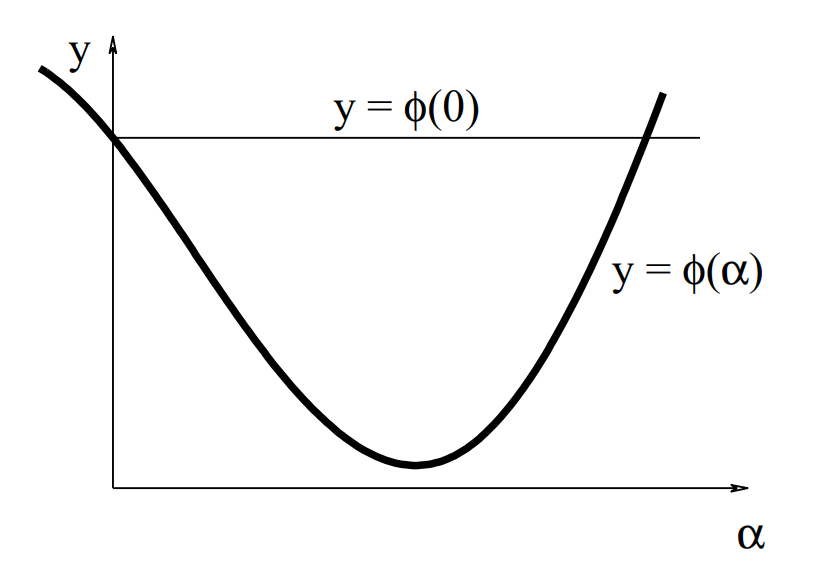
\includegraphics[width=3in]{line-search-cost-function.png}
        \caption{Loss value as a function $\varphi(\alpha)$ of the step length $\alpha$ when $\ve{h}$ is a descent direction \cite{Madsen:2004}.}
        \label{fig:line-search-cost-function}
    \end{figure}

    \item It is tempting to find $\alpha^* = \argmin_{\alpha > 0} \varphi(\alpha)$. This results in an algorithm called {\bf exact line search}. However, this is still a hard optimization problem. Even if we allow ourselves to find a local minimizer instead of the global minimizer, literature still considers it not cost effective.
    
    \item Instead, what people do is {\bf inexact line search} where we produce an $\alpha$ value that is not too short and not too long.
    \begin{itemize}
        \item If $\alpha$ is too short, then $\varphi(0) - \varphi(\alpha)$ might be too small to call it an improvement, implying slow convergence.
        \item If $\alpha$ is too large, then $\varphi(\alpha)$ might be greater than $\varphi(0)$.
    \end{itemize}    
\end{itemize}

\subsubsection{Forms of Line Search Algorithm}

\begin{itemize}
    \item Inexact line search is generally an iterative algorithm.
    \begin{itemize}
        \item Starts with an initial guess $\alpha \gets \alpha^{(0)}$.
        \item Keeps updating the value of $\alpha$ until it satisfies some conditions.
    \end{itemize}

    \item In {\bf backtracking line search} \cite{Norcedal:2006} we start with a large initial guess, say $\alpha^{(0)} = 1$. We keep exponentially decaying the value of $\alpha \gets \rho \alpha$  where $0 < \rho < 1$ until it satisfies some condition. See Algorithm~\ref{algo:backtracking-line-search} for the pseudocode.
    
    \begin{algorithm}[t]
    \begin{algorithmic}
        \State $\alpha \gets \alpha^{(0)}$
        \While {$\alpha$ does not satisfy some conditions}
            \State $\alpha \gets \rho \alpha$
        \EndWhile        
    \end{algorithmic}    
    \caption{Backtracking line search}
    \label{algo:backtracking-line-search}
    \end{algorithm}

    \item In {\bf interval binary search} \cite{Frandsen:2004}, we maintain in interval $[a,b]$ where an $\alpha$ value would be sampled from. After we sample $\alpha$, we would update $[a,b]$ like what we do in binary search: either turning it into $[a,\alpha]$ or $[\alpha,b]$. We keep doing this until our sampled $\alpha$ satisifed some conditions.

    \item In Frandsen~\etal's book \cite{Frandsen:2004}, the authors present a version of interval binary search that has two phases. In the first phase, the interval $[a,b]$ is ``expanded'' until we find something suitable. In the second phase, the binary search kicks in. The pseudocode of the algorithm is given in Algorithm~\ref{algo:interval-binary-search}.
        
    \begin{algorithm}[t]
    \begin{algorithmic}
        \State $k \gets 0$
        \State $a \gets 0$
        \State $b \gets \min\{1, \alpha_{\max}\}$
        \While {($b$ does not satisfy some conditions) {\bf and} $(b \leq \alpha_{\max})$ {\bf and} $(k < k_{\max})$}                        
            \State $a \gets b$
            \State $b \gets \min\{2b, \alpha_{\max}\}$
            \State $k \gets k+1$            
        \EndWhile
        \State $\alpha \gets b$
        \While {($\alpha$ does not satisfy some conditions) {\bf and} $(k < k_{\max})$}
            \State Refine $\alpha$ and $[a,b]$.
            \State $k \gets k+1$
        \EndWhile
        \State \Return $\alpha$
    \end{algorithmic}
    \caption{Interval binary search}
    \label{algo:interval-binary-search}
    \end{algorithm}
\end{itemize}

\subsubsection{Backtracking Armijo Line Search}

\begin{itemize}
    \item The first concrete example of a line search algorithm uses a condition called the ``Armijo condition''~\cite{Norcedal:2006} with the backtracking line search template.
    
    \item The {\bf Armijo condition} is as follow:
    \begin{align*}
        \varphi(\alpha) \leq \varphi(0) + \gamma \cdot \alpha \cdot \varphi'(0)
    \end{align*}
    where $0 < \gamma < 1$, and $\gamma$ is often chosen to be around $10^{-3}$. It is depicted in Figure~\ref{fig:armijo-condition}.

    \begin{figure}
        \centering
        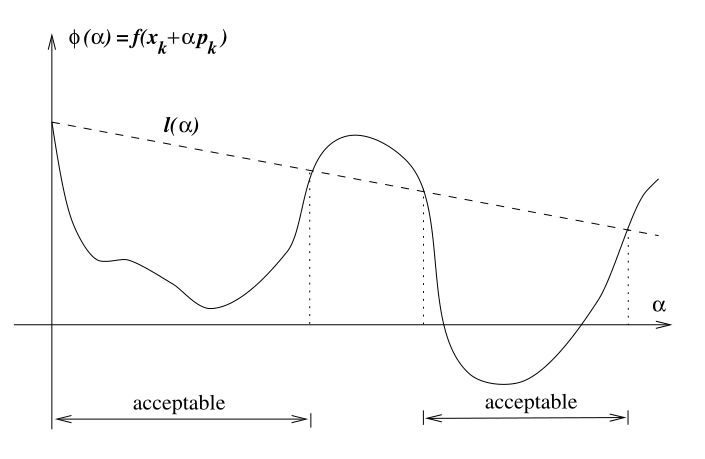
\includegraphics[width=4in]{armijo.png}
        \caption{The Armijo condition.}
        \label{fig:armijo-condition}        
    \end{figure}

    \item We note that the Armijo condition always hold at $\alpha = 0$.

    \item If we graph $\varphi$ as a function of $\alpha$, the Armijo condition requires that we find $\alpha$ such that $(\alpha, \varphi(\alpha))$ is below the line of slope $\gamma \varphi'(0)$ with vertical intercept $\varphi(0)$. In other words, it requires that the loss function decreases by some sufficient amount, determined by $\gamma$.
    \begin{itemize}
        \item As a result, the Armijo condition is sometimes referred to as the {\bf sufficient decrease condition}.        
    \end{itemize}

    \item The pseudocode of the full algorithm is given in Algorithm~\ref{algo:backtracking-armijo-line-search}.
    
    \begin{algorithm}[t]
    \begin{algorithmic}
        \Procedure{Backtracking-Armijo-Line-Search}{}
        \State $\alpha \gets \alpha^{(0)}$
        \While {{\bf not} $\Call{Armijo}{\alpha}$}
            \State $\alpha \gets \rho \alpha$
        \EndWhile
        \State \Return $\alpha$
        \EndProcedure     
        
        \State

        \Procedure{Armijo}{$\alpha$}
            \State \Return $\varphi(\alpha) \leq \varphi(0) + \gamma \cdot \alpha \cdot \varphi'(0)$
        \EndProcedure
    \end{algorithmic}
    \caption{Backtracking Armijo line search}
    \label{algo:backtracking-armijo-line-search}
    \end{algorithm}

    \item The algorithm is gauranteed to terminate because the Armijo condition is always satisfied when $\alpha$ is low enough.
    
    \item A drawback of the algorithm is that there is no conditions that prevent $\alpha$ from being too small.
\end{itemize}

\subsubsection{Interval Binary Search with Wolfe Conditions}

\begin{itemize}
    \item Frandsen \etal\ presents an algorithm they call {\bf soft line search} \cite{Frandsen:2004}, which is basically interval binary search with conditions called the ``Wolfe conditions''.
    
    \item The {\bf Wolfe conditions} \cite{Norcedal:2006} consists of two conditions. The first condition ensures that $\alpha$ is small enough, and the second conditions ensures that $\alpha$ is not too small.
    \begin{itemize}
        \item The first condition is just the Armijo condition with the extra requirement that $\gamma < 0.5$.
        \item The second condition is called the {\bf curvature condition}:
        \begin{align*}
            \varphi'(\alpha) \geq \beta \cdot \varphi'(0)
        \end{align*}
        where $\gamma < \beta < 1$, and $\beta$ is often picked to be much greater than $\gamma$, typically $0.1$. See Figure~\ref{fig:wolfe-curvature-condition}. The curvature condition requires that the gradient increases by some amount, making sure that the picked $\alpha$ yields $\ve{x}$ that is close to a stationary point.
    \end{itemize}

    \begin{figure}
        \centering
        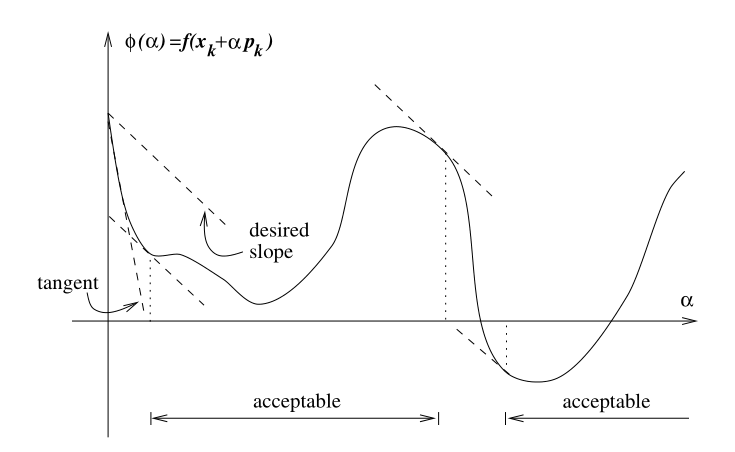
\includegraphics[width=4in]{wolfe-curvature-condition.png}
        \caption{Curvature condition \cite{Cao:2021,Norcedal:2006}.}
        \label{fig:wolfe-curvature-condition}
    \end{figure}

    \item We note that \emph{the curvature condition does not hold at $\alpha = 0$}. If we substitute $\alpha = 0$, we have the condition reads $\varphi'(0) \geq \beta \cdot \varphi'(0)$. In other words, $(1 - \beta) \varphi'(0) \geq 0$. This is false because $1 - \beta > 0$, but $\varphi'(0) < 0$.

    \item To faciliate further discussion, we shall encode the curvature condition as a function in a pseudo programming language like in Algorithm~\ref{algo:curvature-conditions}.
    
    \begin{algorithm}[t]
        \begin{algorithmic}
            \Procedure{Curvature}{$\alpha$}
                \State \Return $\varphi'(\alpha) \geq \beta \cdot \varphi'(0)$
            \EndProcedure            
        \end{algorithmic}
        \caption{The curvature condition and its strict version, encoded as functions in a pseudo programming language.}
        \label{algo:curvature-conditions}
    \end{algorithm}

    \item The pseudocode for the algorithm in given in Algorithm~\ref{algo:interval-binary-search-with-wolfe-conditions}.    
    
    \begin{algorithm}[t]        
        \begin{algorithmic}
            \Procedure{Interval-Binary-Search-With-Wolfe-Conditions}{}
            \If {$\varphi'(0) \geq 0$}
                \State \Return $0$
            \EndIf
            \State $k \gets 0$
            \State $a \gets 0$
            \State $b \gets \min\{1, \alpha_{\max}\}$
            \While {$\Call{Armijo}{b}$ {\bf and} ({\bf not} $\Call{Curvature}{b}$) {\bf and} $(b \leq \alpha_{\max})$ {\bf and} $(k < k_{\max})$}                        
                \State $a \gets b$
                \State $b \gets \min\{2b, \alpha_{\max}\}$
                \State $k \gets k+1$            
            \EndWhile
            \State $\alpha \gets b$
            \While {({\bf not} $\Call{Armijo}{\alpha}$) {\bf or} ({\bf not} $\Call{Curvature}{\alpha}$) {\bf and} $(k < k_{\max})$}
                \State $\alpha, a, b \gets \Call{Refine}{\alpha,a,b}$
                \State $k \gets k+1$
            \EndWhile
            \If $\varphi(\alpha) \geq \varphi(0)$
                \State $\alpha \gets 0$
            \EndIf
            \State \Return $\alpha$            
            \EndProcedure                                    

            \State

            \Procedure{Refine}{$\alpha, a, b$}
                \State $D \gets b - a$
                \State $c \gets (\varphi(b) - \varphi(a) - D \phi'(a)) / D^2$
                \If {$c < 0$}
                    \State $\alpha \gets a - \varphi'(a) / (2c)$
                    \State $\alpha \gets \min\{ \max\{ \alpha, a + 0.1D\}, b - 0.1D \}$
                \Else
                    \State $\alpha \gets (a+b) / 2$
                \EndIf
                \If {$\Call{Armijo}{\alpha}$}
                    \State $a \gets \alpha$
                \Else
                    \State $b \gets \alpha$                    
                \EndIf
                \State \Return $\alpha, a, b$
            \EndProcedure
        \end{algorithmic}
        \caption{Interval binary search with Wolfe conditions}
        \label{algo:interval-binary-search-with-wolfe-conditions}
    \end{algorithm}

    \item The algorithm is quite complicated. There are two while loops.
    \begin{itemize}
        \item The first while loop finds an interval $[a,b]$ to be used in the binary search.
        \item The second while loop implements the binary search.
    \end{itemize}

    \item The loop invariance of the second while loop is has the following three conditions.
    \begin{enumerate}
        \item $\alpha \in [a,b]$.
        \item $\Call{Armijo}{a}$ {\bf and} ({\bf not} $\Call{Curvature}{a}$).
        \item ({\bf not} $\Call{Armijo}{b}$) {\bf or} $\Call{Curvature}{b}$.
    \end{enumerate}
    In other words, we want $a$ to too small, and $b$ to be too large or sufficiently large. Because $\alpha$ is between something too small and something large enough or too large, $\alpha$ has a chance to be just right.
    
    \item The first loop updates $[a,b]$ until the we find an interval that satisfies the last two coditions above.
    
    \begin{itemize}
        \item Setting $a = 0$ at before the first loop makes sure that both $\Call{Armijo}{a}$ and ({\bf not} $\Call{Curvature}{a}$) hold. However, we don't know about what conditions $b$ satisfies at that point, and the first loop would find a $b$ that violates at least one of them.
    
        \item We can see that the updates in the first loop are correct. If we choose to update $a \gets b$, it means that the predicate of the while loop is true. This means that $\Call{Armijo}{b}$ and ({\bf not} $\Call{Curvature}{b}$) hold, and we are free to set $a$ to $b$.            
    \end{itemize}
    
    \item Let's take a closer look at the second loop.
    \begin{itemize}
        \item         
    \end{itemize}
\end{itemize}


\bibliographystyle{acm}
\bibliography{nonlinear-least-square-algo}
\end{document}